\chapter{X-ray principles}\label{chap:xray_appendix}
\renewcommand{\papertitle}{X-ray principles}
\markboth{}{}
This chapter is taken from my own master thesis from 2010 and describes the principles of X-ray reflection from imperfect surfaces and interfaces.

Anders C. Jakobsen, Developing Supermirror Optics for Hard X-rays, \emph{Master thesis}, University of Copenhagen, 2010.

\newpage\mbox{} % Blank side s� artiklen starter p� et ulige sidetal
\markboth{\papertitle}{}

% \section{X-ray principles}
The development of multilayer mirrors for X-ray focusing requires the ability to measure the properties of the deposited films. A number of techniques can be used, but by far the most practical is X-Ray Reflectometry (XRR) that allows for relatively fast ($\sim$ 20 mins. in our setup) non-destructive measurements and gives information about thicknesses, densities and interlayer imperfections.

\section{Reflection from a surface}
An X-ray photon propagating through one medium and hitting the surface of another medium will interact with the surface by changing direction, either as reflection or refraction. The principle of refraction is explained by \emph{Snell's Law}
\begin{eqnarray}
	n_1 \cos{\theta_1} = n_2 \cos{\theta_2}
\end{eqnarray}

where $n_1$ and $n_2$ are the refractive indexes of the first and second medium respectively. $\theta_1$ and $\theta_2$ are the grazing angle of the incident photon and grazing angle of refracted photon respectively.\\

For an incident plane harmonic wave propagating in the direction $\mathbf{K}$, the electric field can be described as
\begin{eqnarray}
	\mathbf{E} = E_0 \mathrm{e}^{i(\mathbf{K}\cdot \mathbf{r}-\omega t)}
\end{eqnarray}

with amplitude $E_0$. The magnetic field in the plane harmonic wave, $\mathbf{B}$, is perpendicular to the electric field.\\

There are two polarization modes when considering a plane harmonic wave incident on a surface, either the polarization is Transverse Electric (TE) or Transverse Magnetic (TM). In the TE mode, the electric field is perpendicular to the plane of incidence, and in the TM mode the magnetic field is perpendicular to the plane of incidence. Any combination of polarization of the two modes can be considered a superposition of the two, so it is enough to look at only the TE and TM modes. And since for small angle grazing incidence X-ray cases the two are nearly identical\cite{pedrotti:1993}, only the TE mode will be considered from here on. \\

As the incident wave hits the surface it can either reflect or refract and the electric field of the reflected, $E_r$, and refracted, $E_t$, waves are
\begin{eqnarray}
	\mathbf{E_r} & =  & E_r \mathrm{e}^{i(\mathbf{K}\cdot \mathbf{r}-\omega t)},\\
	\mathbf{E_t} & =  & E_t \mathrm{e}^{i(\mathbf{K}\cdot \mathbf{r}-\omega t)}.
\end{eqnarray}

The relation between reflection, refraction and incident wave is described by the reflectivity amplitude, $r$, and transmittivity amplitude, $t$. They are calculated from the electric field amplitudes and their projection parallel to the surface
\begin{eqnarray}
	E \sin{\theta} - E_r \sin{\theta} &=& n E_t \sin{\theta_t}.
\end{eqnarray}

and provide the Fresnel equations
\begin{eqnarray}\label{fresneleq}
	r & \equiv & \frac{E_r}{E} = \frac{\sin{\theta}-n \sin{\theta_t}}{\sin{\theta}+n \sin{\theta_t}}, \\
	t & \equiv & \frac{E_t}{E} = \frac{2\sin{\theta}}{\sin{\theta}+n \sin{\theta_t}}
\end{eqnarray}

that describes the reflectivity and transmittivity from an interface between a medium with refractive index of unity (vacuum/air) and another medium with refractive index $n$.

\section{Reflection from a thin film}
Further evolving the Fresnel equation to describe $r$ and $t$ from an interface between two mediums with refractive indexes $n_i$ and $n_j$ yields
\begin{eqnarray}
	r_{ij} & \equiv & \frac{E_i^{'}}{E_i} = \frac{n_i\sin{\theta_i}-n_j \sin{\theta_j}}{n_i\sin{\theta_i}+n_j \sin{\theta_j}}, \label{reflectivitetinterface}\\
	t_{ij} & \equiv & \frac{E_t}{E_i} = \frac{2 n_i\sin{\theta_i}}{n_i\sin{\theta_i}+n_j \sin{\theta_j}}.\label{transmittivity}
\end{eqnarray}

Here $E_i$ is the electric field amplitude incident on the interface in medium $i$ and $E_i^{'}$ is the reflected electric field amplitude in medium $i$. $E_j$ is the refracted electric field amplitude in medium $j$.\\

For a thin film on a substrate, there are three mediums: First air ($n_0$), then film ($n_1$) and finally substrate ($n_s$). An incident X-ray photon acting on a thin film have an infinite number of ways to interact with the interfaces. Either the photon is reflected from the first layer, so $r_{01} = 1$, or it is transmitted through the first layer and reflected from the next, or transmitted, then reflected, then reflected and so on. All those possibilities are described by a geometric series
\begin{eqnarray}
	r_{\mathrm{thin film}} = r_{01} + t_{01}t_{10}r_{1s}\mathrm{e}^{2 i \beta_i}\sum_{m=0}^{\infty}(r_{10}r_{12}\mathrm{e}^{2 i \beta_i})^m
\end{eqnarray}

where $\mathrm{e}^{2i\beta_i}$ is a phase factor to correct the phase of the waves before being added up and $\beta = 2 \pi d_i n_i \sin{\theta_i}\lambda^{-1}$. Noting that $\sum_{m=0}^{N}k^n = \frac{1 - k^n}{1-k}$ becomes $\sum_{m=0}^{\infty}k^n = \frac{1}{1-k}$ for $|k| < 1$, the series can be simplified to
\begin{eqnarray}
	r_{\mathrm{thin film}} = r_{01} + t_{01}t_{10}r_{1s}\mathrm{e}^{2i\beta_i}\frac{1}{1-r_{10}r_{12}\mathrm{e}^{2i\beta_i}}
\end{eqnarray}

and finally give
\begin{eqnarray}
	r_{\mathrm{thin film}} = \frac{r_{01} + r_{12}\mathrm{e}^{2i\beta_i}}{1-r_{10}r_{12}\mathrm{e}^{2i\beta_i}} \label{slabapprox}
\end{eqnarray}

\section{Reflection from multilayers}
For calculating the reflectivity from a multilayer stack a method such as the Kinematical approximation can be used. But the approximation have the downside of only being able to calculate for multilayers where the bilayer thickness (d-spacing) is constant throughout the multilayer stack. \\
Since the development of X-ray optics involves making multilayers where the d-spacing change through the stack, it is more appropriate to compute an iterative model using the formula just derived in Eq. (\ref{slabapprox}) . The software used in modeling specular reflectivity from a multilayer is IMD\cite{Windt:1998p3071}. It takes the two formulas
\begin{eqnarray}\label{fresnelcoef}
	r_i &=& \frac{r_{ij}+r_j\mathrm{e}^{2 i \beta_i}}{1+r_{ij}r_j\mathrm{e}^{2 i \beta_i}},\\
	t_i &=& \frac{t_{ij}t_j\mathrm{e}^{2 i \beta_i}}{1+r_{ij}r_j\mathrm{e}^{2 i \beta_i}}\\
\end{eqnarray}

to calculate the $i$'th layer where $r_{ij}$ is Eq. (\ref{reflectivitetinterface}) and $t_{ij}$ is Eq. (\ref{transmittivity}). Since the $j$'th layer is the layer below $i$, the software calculation can start from the bottom layer, the substrate, where there is no reflectivity from below. From the bottom layer, the software works it way up recursively through each layer, adding up the reflectivity and transmittivity. That is the Paratt recursive method\cite{Parratt:1954p5110}.\\
The energy reflected from or transmitted through the film is denoted as the reflectance $R$ and transmittance $T$
\begin{eqnarray}
	R &=& |r|^2,\\
	T &=& \mathrm{Re}\Bigg\{\frac{n_s \sin{\theta_s}}{n_a \sin{\theta_a}}\Bigg\}|t|^2.
\end{eqnarray}

The IMD software approximates the absorptance, $A$, using $R$ and $T$
\begin{eqnarray}
	A = 1-R-T
\end{eqnarray}

where A is the energy absorbed by the entire film.

\section{Reflectivity changes due to imperfections in the interface}
In experimental cases, the interface between two mediums, or materials, is not completely smooth. The imperfections can be distinguished into two types. Either by atoms in the structure that have been deposited unevenly to create 'hills' and 'valleys' in the surface, which is called pure roughness, $\sigma_p$. The other type is diffuse roughness, $\sigma_d$, caused by diffusion of atoms from one material into another.\\
To describe the roughness, the interface can be seen as not an abrupt change of refractive index, but as a profile function, $p(z)$\cite{Stearns:1989p5096}, that takes the normalized average value of the dielectric function, $\varepsilon(\mathbf{x})$, in the $z$ direction, where
\begin{eqnarray}
	p(z) = \frac{\int \int \varepsilon(\mathbf{x})dxdy}{(\varepsilon_i-\varepsilon_j)\int \int dxdy}, \\
	\varepsilon(\mathbf{x}) = \Bigg\{
	\begin{array}{rl}
		\varepsilon_i, & z \rightarrow + \infty \\
		\varepsilon_j, & z \rightarrow - \infty \\
	\end{array}.
\end{eqnarray}

Taking the Fourier transform of $dp/dz=w(z)$ gives $\tilde{w}(s)$, where $s = 4 \pi \sin{\theta}/\lambda$. As Stearn found out, multiplying the Fresnel coeffiecients from Eq. (\ref{fresnelcoef}) with $\tilde{w}(s)$ gives the approximate reflectance including loss from imperfect interfaces. That gives the modified Fresnel coefficients used by IMD:
\begin{eqnarray}
	r_{ij}^{'} = r_{ij} \tilde{w}(s).
\end{eqnarray}

The most commonly used interface profile, $p(z)$, is the error function
\begin{eqnarray}
	p(z) = \frac{1}{\sqrt{\pi}}\int_{-\infty}^z \mathrm{e}^{-t^2/(2\sigma_{rms}^{2})}dt
\end{eqnarray}

which after taking the Fourier transform of $dp/dz$ becomes
\begin{eqnarray}\label{interfacefunction}
	\tilde{w}(s) = \mathrm{e}^{-s^2\sigma_{rms}^2/2}.
\end{eqnarray}\\

The width of the interface function is denoted by $\sigma_{rms}$ that is the root mean square of $\sigma_p$ and $\sigma_d$, so
\begin{eqnarray}
	\sigma_{rms} = \sqrt{\frac{\sigma_p^2 + \sigma_d^2}{2}}.
\end{eqnarray}

\section{Diffuse reflection}\label{diffuserefl}
In the previous section only specular reflection was covered and dealt with by reducing the problem to a one-dimensional one without worrying about scattering. In case of roughness, there was merely an approximate factor to account for loss of reflection.\\
Roughness in an interface will cause scattering outside the specular reflection, which can be modeled either using the Born Approximation (BA) or Distorted Wave Born Approximation (DWBA)\cite{Sinha:1988p5102}. The regular BA is suitable for looking at scattering away from the critical angle, where scattering is considered a weak interaction and multiple refraction effects are negligible. When looking at multilayers, the BA is not suitable since it does not take multiple reflections into account.\\
The DWBA is more suitable for multilayers, where total external and internal reflections near the critical angle are taken care of. Every imperfect interface is regarded as a perturbation. Sinha et al.\cite{Sinha:1988p5102} worked out the DWBA for singlelayer and later the model was expanded to include multilayer systems\cite{Stearns:1998p5375,Kopecky:1995p5468,Holy:1993p5469}. In this section the formulas will not be derived, but the final formula presented and explained.\\

The measured intensity in a scattering experiment is explained by
\begin{eqnarray}
	I = I_0 \int_{\Omega_{detector}} \frac{d\sigma}{d\Omega} d\Omega.
\end{eqnarray}

where $I$ is the measured intensity, $I_0$ the incident intensity and $\frac{d\sigma}{d\Omega}$, the differential cross section. For non-specular reflectivity, the incoherent differential cross section is used, as derived for multilayers by Holy et al.\cite{Holy:1993p5469}

\begin{eqnarray}\label{holyeq}
	\Bigg(\frac{d\sigma}{d\Omega}\Bigg)_I &=&\frac{Sk^4}{16\pi^2}\sum_{i=1}^N |n_{i}^2 - n_{i+1}^2|^2  \nonumber \\
	 &\times&|(t_{1,i+1}t_{2,i+1}+r_{1,i+1}r_{2,i+1})\mathrm{e}^{\frac{-(\sigma_i q_{0z,i+1})^2}{2}} \nonumber  \\
	 &+&(t_{1,i+1}r_{2,i+1}+t_{2,i+1}r_{1,i+1})\mathrm{e}^{\frac{-(\sigma_i q_{1z,i+1})^2}{2}}|^2 \\
  &\times& C_i^{'} (q_x,q_y)
\end{eqnarray}

which is the simplified version applicable when $|q_{z,i+1}\sigma_2|^2 << 1$. The first factor contains the area $S$ hit by the incident beam and the wave number $k = 2\pi/\lambda$. Next is the sum that iterates over all $N$ layers from bottom layer up. The factor $|n_{i}^2 - n_{i+1}^2|$ takes the square of the index of the current layer and subtracts the square of the index of the layer above.\\
Next is the Fresnel equations (Eq. (\ref{fresneleq})) which are multiplied by a modified interface function similar to Eq. (\ref{interfacefunction}) except the use of $q_{0z,i+1}$ and $q_{1z,i+1}$.\\
The two wave vector transfers correspond to two different processes that occurs during diffuse scattering. The term $t_{1,i+1}t_{2,i+1}$ express the scattering from the transmitted wave with amplitude $t_{1,i+1}$ into the wave with amplitude $t_{2,i+1}$. The wave vector change corresponding to that interaction is $\mathbf{q}_{0,i+1} = \mathbf{K}_{2,i+1}-\mathbf{K}_{1,i+1}$. Refer to figure \ref{fig:holykvector}.\\
And for $t_{1,i+1}r_{2,i+1}$, it is the scattering from the transmitted wave with amplitude $t_{1,i+1}$ into the reflected wave with amplitude $r_{2,i+1}$ and the wave vector transfer for that is $\mathbf{q}_{1,i+1} = \mathbf{K}_{2,i+1}^{'}-\mathbf{K}_{1,i+1}$.

\begin{figure}[!ht] % holykvector
	\centering
		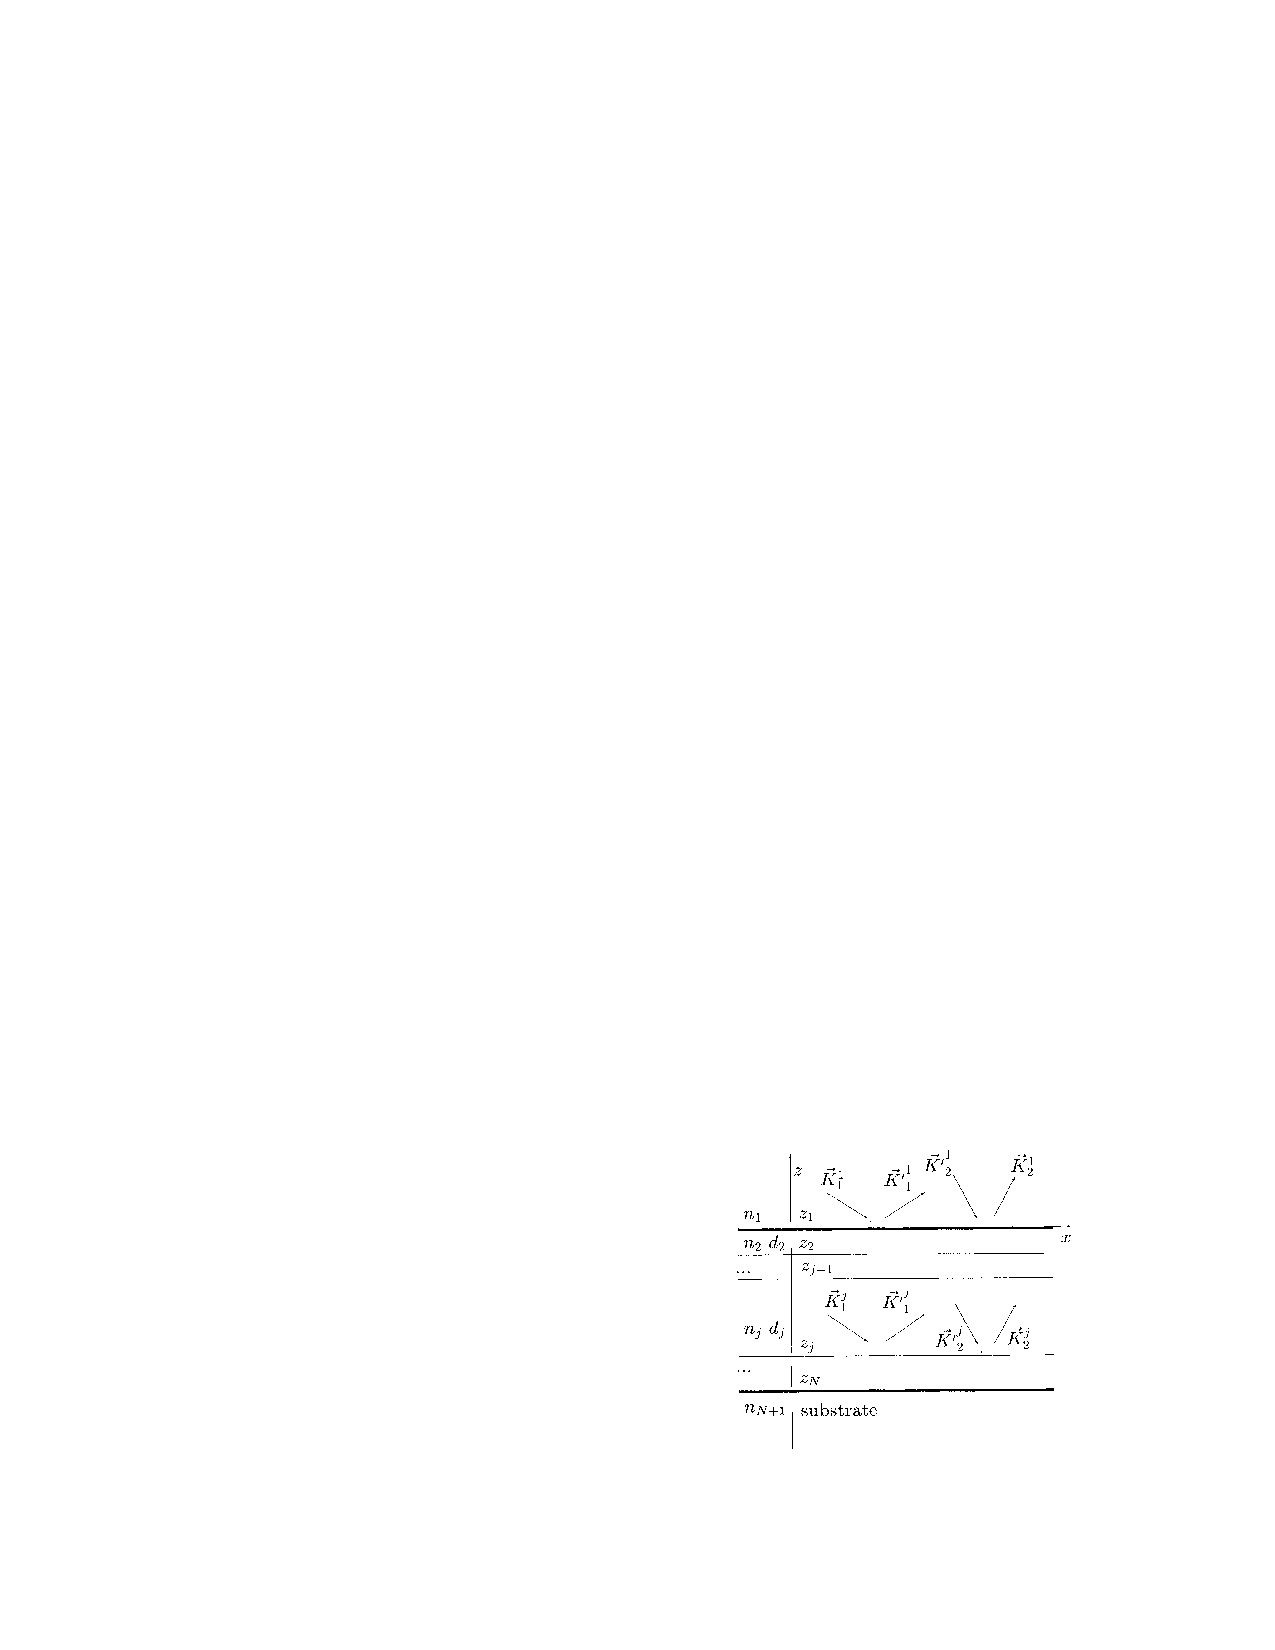
\includegraphics[height=2.2in]{figures/xray_app/holykvector.pdf}
	\caption{Cross section of $N$-layer multilayer on substrate with visualization of wave vectors on the surface and in the $j$'th layer. From \cite{Holy:1993p5469}.}
	\label{fig:holykvector}
\end{figure}

The last part in Eq. (\ref{holyeq}), $C_i^{'} (q_x,q_y)$, is the two dimensional Fourier transform of the correlation function, $C_i$
\begin{eqnarray}
	C_i^{'} (q_x,q_y) &=& \int_S dxdy C_i(x,y)\mathrm{e}^{-i(xq_x +yq_y)}.
\end{eqnarray}

The correlation function is often described with a statistical distribution of a self-affine fractal-like surface\cite{Sinha:1988p5102}
\begin{eqnarray}
	C_i (x,y) = \sigma^2 \mathrm{e}^{-(\rho/\xi)^2h}
\end{eqnarray}

where $\sigma$ is the rms roughness of the surface and $\xi$ is a lateral correlation length which is an expression for how large an area is needed to measure before $\sigma$ is constant. If the roughness is periodic along the surface, $\xi$ is the length of the period. $h$ is the Hurst parameter that describes the jaggedness of the surface between 0 and 1. For $h=0.5$ the function becomes exponential and for $h=1$ it is Gaussian. So the higher the Hurst parameter, the smoother the surface.\\

The software used for modeling diffuse reflectivity is BEDE\cite{Wormington:1992p5128}, which uses Eq. (\ref{holyeq}) for the off-specular part. In this work, measurements of diffuse reflectivity were done by transverse scans, where the sum of the ingoing angle, $\theta_{I_0}$, and outgoing angle, $\theta_I$, is constant ($\theta_{I_0} + \theta_I=\mathrm{constant}$). \\

\begin{figure}[!ht] % double reflected
	\centering
		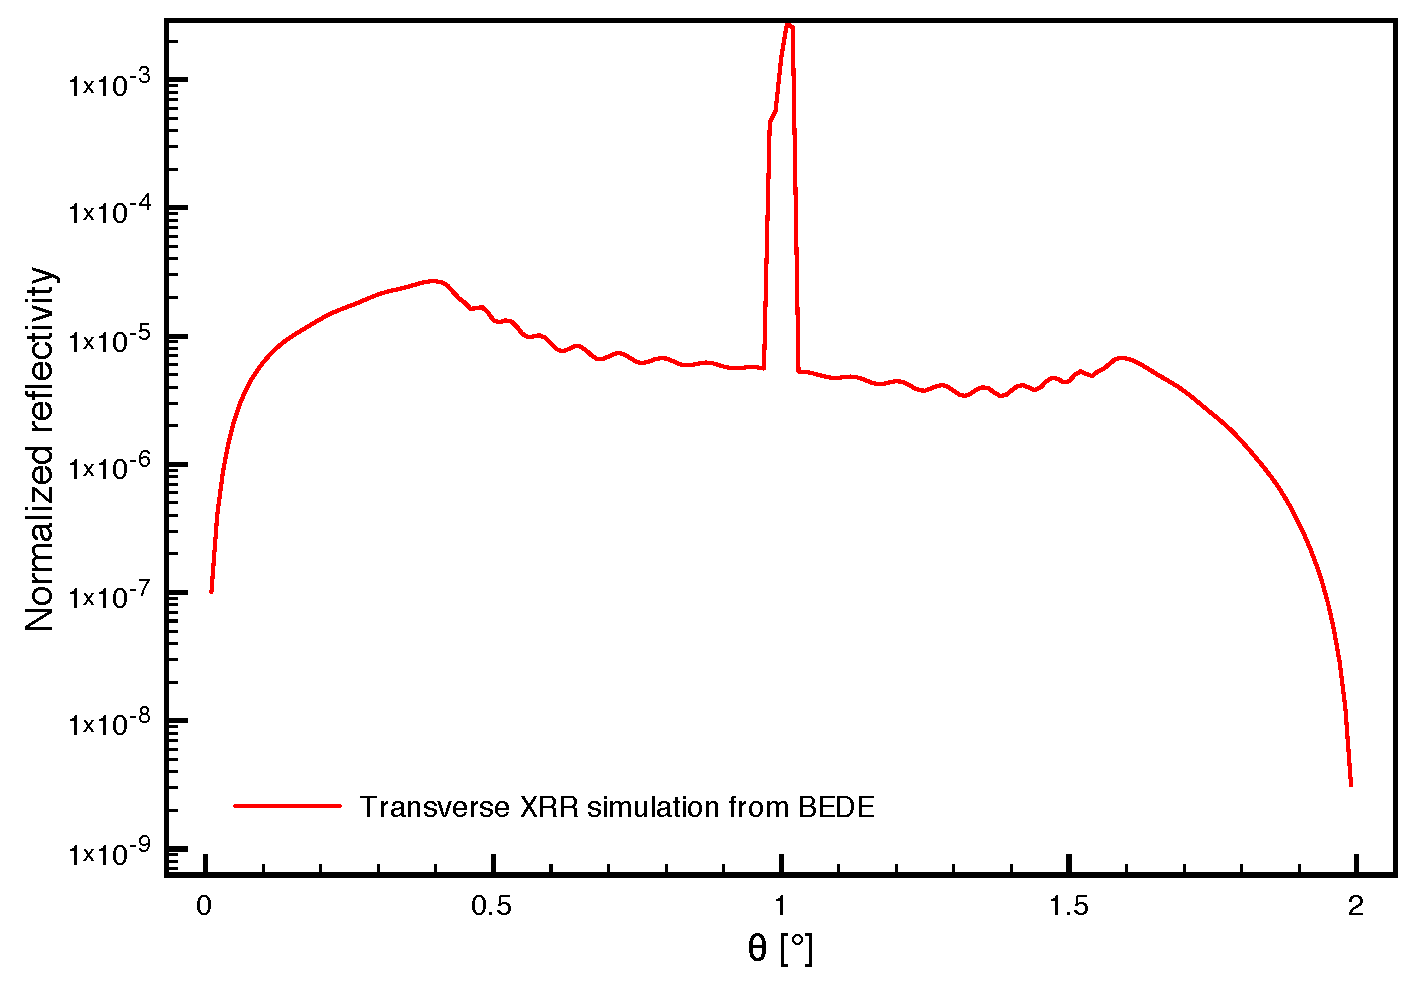
\includegraphics[height=2in]{figures/xray_app/transverse.pdf}
	\caption{Simulation of a transverse XRR scan calculated in BEDE of a 400 \AA\ W singlelayer on a silicon substrate with roughness of 4 \AA, correlation length of 200 \AA\ and Hurst parameter of 0.7. }
	\label{fig:transverse}
\end{figure}

An example of a simulated transverse reflection can be seen in figure \ref{fig:transverse}. The peaks on both sides of the graph are Yoneda peaks\cite{Yoneda:1963p5493} and arise from multiple scattering processes when either $\theta_{I_0}$ or $\theta_I$ equals the critical angle, $\theta_c$.
